\chapterimage{/99/head.jpg} % Chapter heading image
\chapter{Dalla letteratura}\label{last:ch}

Una galleria di articoli e belle immagini per spunti di approfondimento. Ora tocca a voi...




\section{Annual Review of Astronomy and Astrophysics}
\subsection*{Ferreira - Cosmological Tests of Gravity (2019)}
\url{https://doi.org/10.1146/annurev-astro-091918-104423}

\begin{figure}[H]
    \centering
    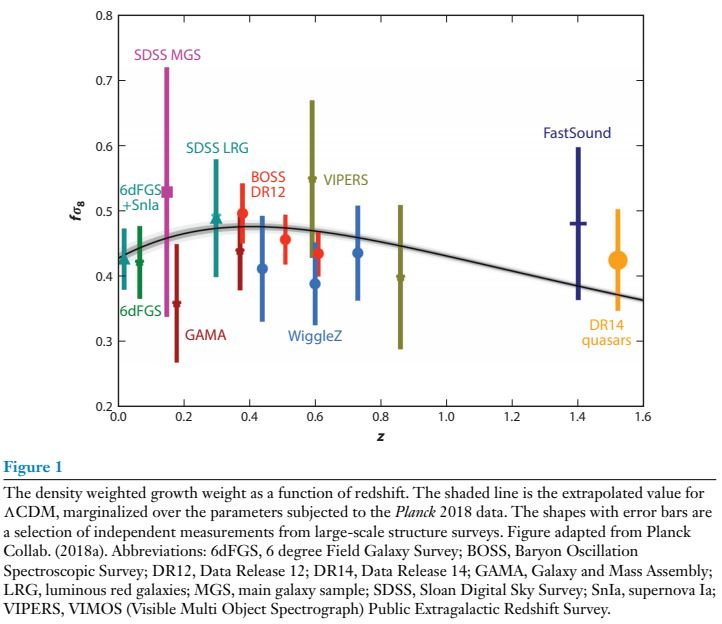
\includegraphics[width=.75 \textwidth]{Pictures/99/ei2018-1.jpg}
\end{figure}
\begin{figure}[H]
    \centering
    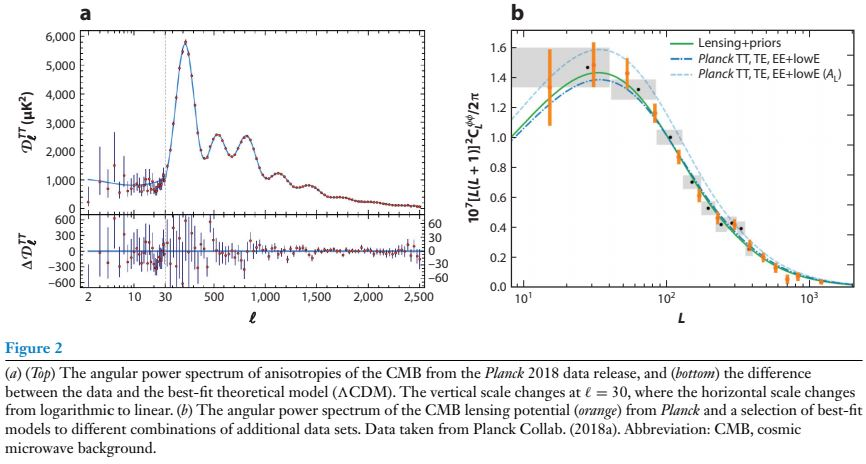
\includegraphics[width=.86 \textwidth]{Pictures/99/ei2018-2.jpg}
\end{figure}
\begin{figure}[H]
    \centering
    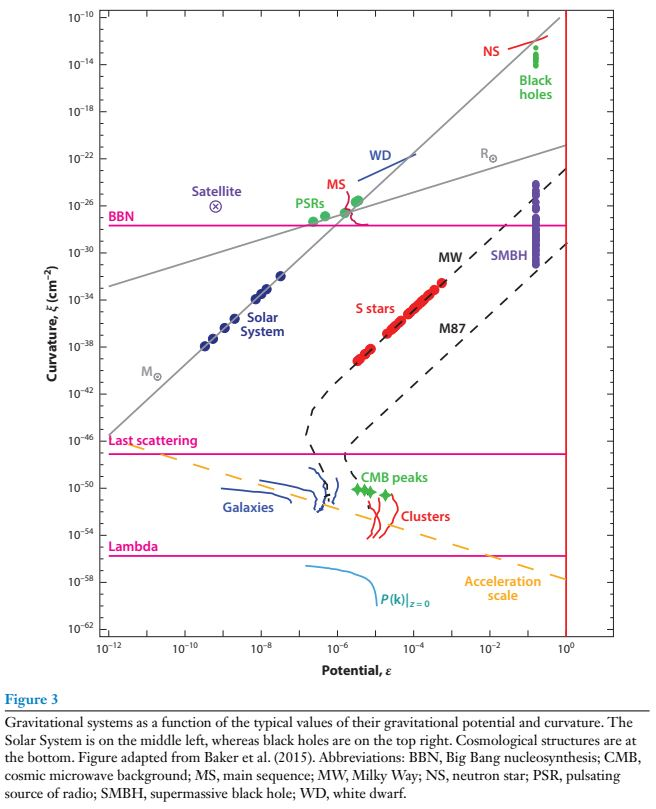
\includegraphics[width=.75 \textwidth]{Pictures/99/ei2018-3.jpg}
\end{figure}

\subsection*{Einasto - Cosmology Paradigm Changes (2018)}
\url{https://doi.org/10.1146/annurev-astro-081817-051748}


\subsection*{Mandelbaum - Weak Lensing for Precision Cosmology (2018)}
\url{https://doi.org/10.1146/annurev-astro-081817-051928}
\begin{figure}[H]
    \centering
    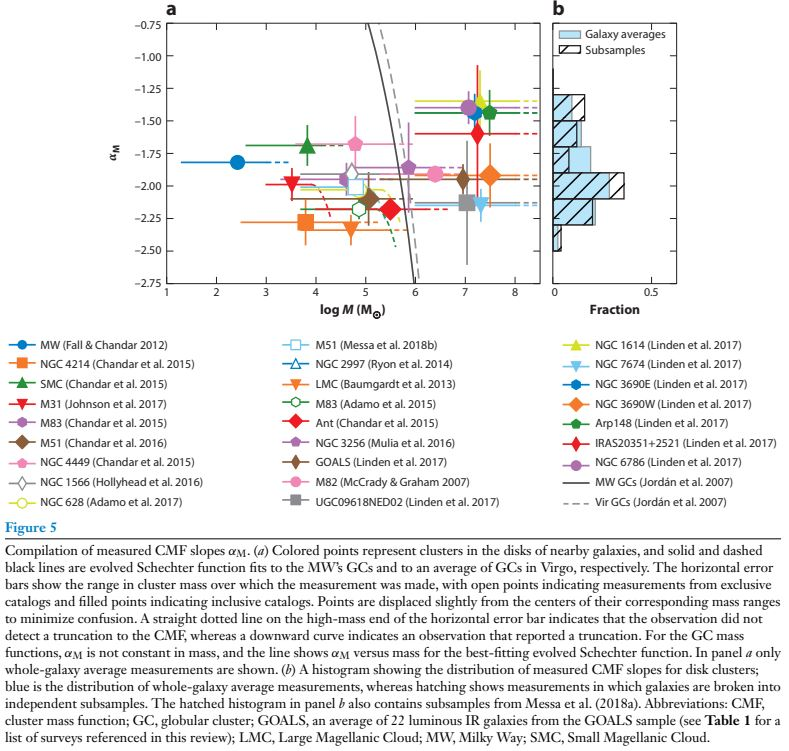
\includegraphics[width=.85 \textwidth]{Pictures/99/ei2018-4.jpg}
\end{figure}

\subsection*{Bullock \& Boylan-Kolchin - Small-Scale Challenges to the $\Lambda$CDM Paradigm (2017)}
\url{https://doi.org/10.1146/annurev-astro-091916-055313}

\subsection*{Frebel \& Norris - Near-Field Cosmology with Extremely Metal-Poor Stars (2015)}
\url{https://doi.org/10.1146/annurev-astro-082214-122423}




\newpage
\section{Hubble constant $H_0$}

\subsection*{Tensions between the Early and the Late Universe}
\url{https://doi.org/10.1038/s41550-019-0902-0}
\begin{figure}[H]
    \centering
    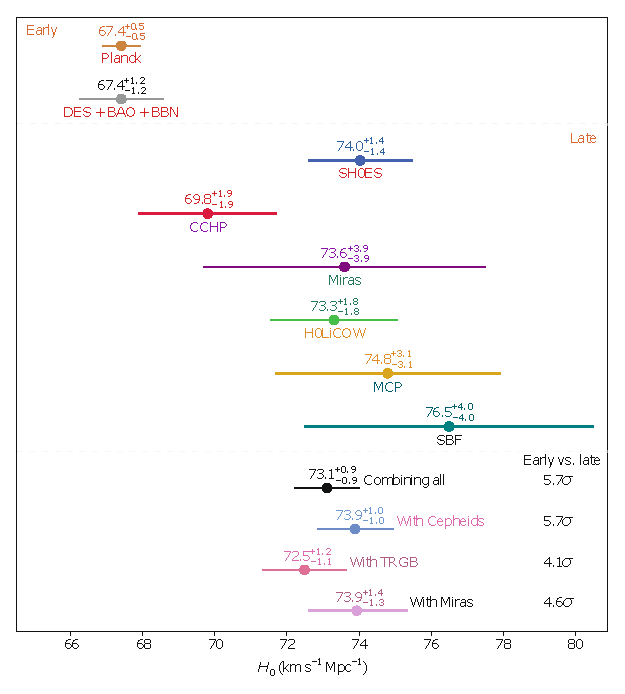
\includegraphics[width=.85 \textwidth]{Pictures/99/Tensions.eps}
    \caption{Compilation of Hubble constant predictions and measurements taken from the recent
    literature.}
\end{figure}



\section{Dark Matter}

\subsection*{Warm dark matter chills out: constraints on the halo mass function and the free-streaming length of dark matter with eight quadruple-image strong gravitational lenses}
\url{https://doi.org/doi:10.1093/mnras/stz3480}



\section{Simulations}


\subsection*{Cosmological baryon transfer in the SIMBA simulations}
\url{https://doi.org/doi:10.1093/mnras/stz3428}